\newpage
\chapter{Evaluation}

The following features of LoYiW project will be evaluated in this chapter, by running on the network devices, get the following results: 

The following figure shows the result on the browser of mobile device. The first line of the result is MAC - Device - Dict, it display only once,when the program run first time. The target IP on the result means IP address of AP, which is connected to the mobile device. The final line of the result is the MAC address of the AP. The result shows that,the AP has been found, which is connected to the mobile device.

\begin{figure}[!ht]
	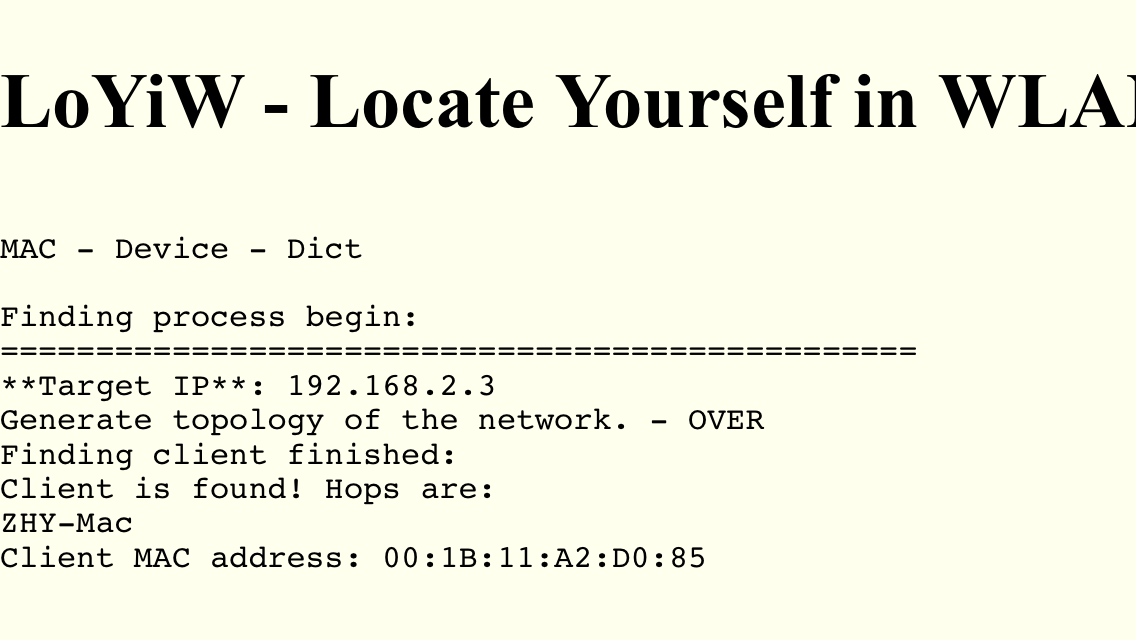
\includegraphics{images/loyiw-run1}
	\caption{Result when the mobile phone is connected to the D-Link}
\end{figure}

The next figure shows that, a device roams from one AP to the next AP,  A new AP information of the target IP and the MAC address is on the result page.

\begin{figure}[!ht]
	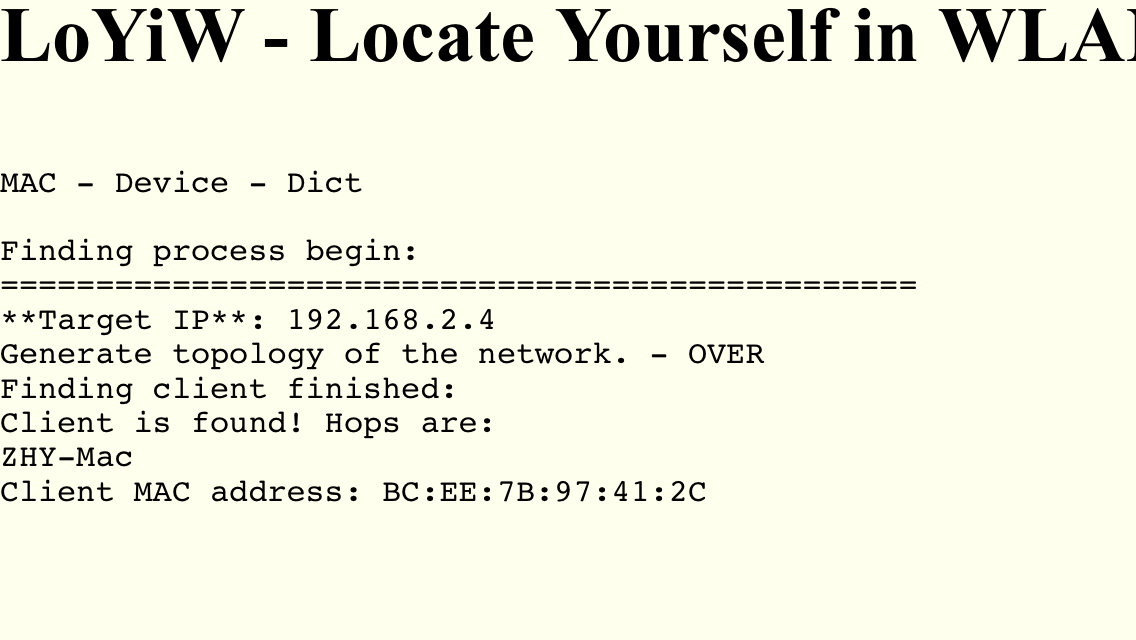
\includegraphics{images/loyiw-run2}
	\caption{Result when the mobile phone is connected to the ASUS RT-N16}
\end{figure}



SNMP tables
Access SNMP table

SNMP contains a lot of tables.
Used tables in this program are listed below:
ipNetToMediaTable - The IPv4 Address Translation table used for mapping from
IPv4 addresses to physical addresses.

This table has been deprecated, as a new IP version-neutral table has been added. It is loosely replaced by the ipNetToPhysicalTable.
List media interfaces
There are different ways to get the media interfaces of the devices.
Using the ifTable command to list

\begin{lstlisting}[language=bash]
$ snmptable -v 2c -c public localhost ifTable
\end{lstlisting}

\begin{lstlisting}[caption={iptables contains too many fields, so it is too long to be displayed as normal source code. The following fields are not important, so they are displayed here: ifAdminStatus ifOperStatus  ifLastChange ifInOctets ifInUcastPkts ifInNUcastPkts ifInDiscards ifInErrors ifInUnknownProtos ifOutOctets ifOutUcastPkts ifOutNUcastPkts ifOutDiscards ifOutErrors ifOutQLen ifSpecific}]
ifIndex ifDescr ifType ifMtu ifSpeed ifPhysAddress
1       lo0 softwareLoopback 16384          0            
2      gif0        ieee80212  1280          0   
3      stf0   hippiInterface  1280          0    
4       en0   ethernetCsmacd  1500 1000000000 0:b0:35:f3:cd:28
5       en1   ethernetCsmacd  1500    5250000 0:15:9e:97:55:81
6       fw0         ieee1394  4078   10000000 0:30:62:ff:fe:e9:fb:b8
7      p2p0   ethernetCsmacd  2304   10000000 0:15:9e:97:55:81
8 bridge100           bridge  1500          0 0:b0:35:3f:f4:64 
\end{lstlisting}

Access the iftable, could 




\subsection{}